\documentclass[aspectratio=169,11pt]{beamer}
\usepackage{fontspec}
\setsansfont{DejaVu Sans}
\usepackage{polyglossia}
\setdefaultlanguage{russian}
\usepackage{graphicx}
\definecolor{ink}{HTML}{17324D}
\definecolor{accent}{HTML}{277D77}
\setbeamercolor{normal text}{fg=ink,bg=white}
\setbeamertemplate{navigation symbols}{}
\setbeamertemplate{footline}{}
\setbeamerfont{normal text}{size=\small}
\setbeamersize{text margin left=.55cm,text margin right=.55cm}
\begin{document}
\begin{frame}[t,plain]
{\fontsize{15}{18}\selectfont\bfseries Обучение роутера: исправления и вред}\par
\vspace{.1cm}
{\fontsize{8}{10}\selectfont Anastasia Shlopak \hfill Руководитель: Archil Maysuradze, PhD}\par
\vspace{.14cm}
{\fontsize{10}{12}\selectfont\textbf{Цель:} выбор обучения роутера по данным, паре моделей и бюджету.}\par
\vspace{.12cm}
{\fontsize{9}{11}\selectfont\textcolor{accent}{Контроль:} фиксируем экспертов и признаки; меняем объём и состав train.}\par
\vspace{.03cm}
{\centering
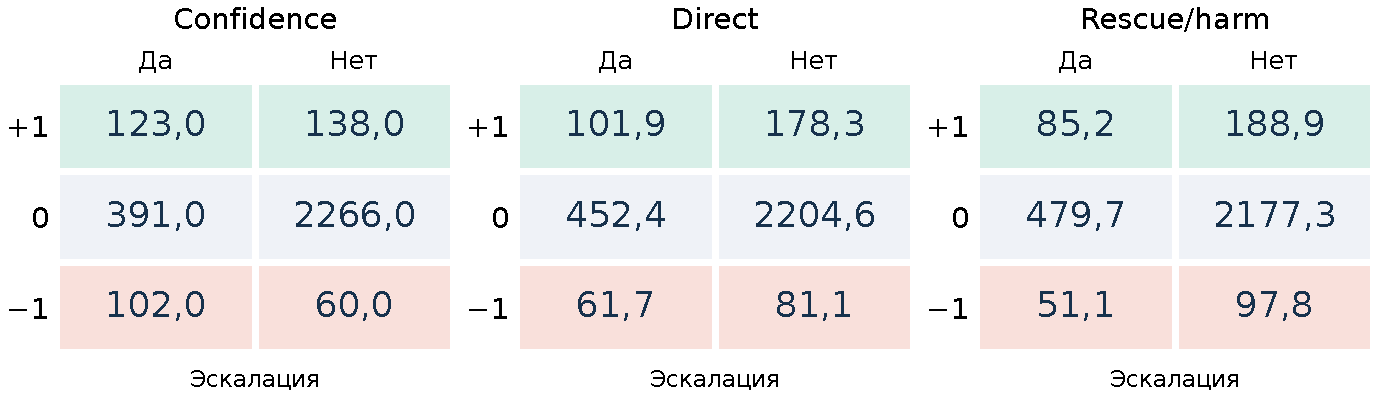
\includegraphics[height=3.0cm]{../paper/figures/decision_profiles.pdf}
\par}
\vspace{-.2cm}
{\fontsize{7.5}{9}\selectfont BANKING77: TF--IDF $\to$ BERT-tiny; 20\% вызовов; fit 1000/dev 500; 10 обучений.}\par
\vspace{.13cm}
{\fontsize{8.5}{10.5}\selectfont Строки: $+1$ --- выбор лучше альтернативы;
$-1$ --- хуже; $0$ --- правильность совпадает.}\par
\vspace{.17cm}
{\fontsize{10}{12}\selectfont\textbf{Наблюдение:} Events реже исправляет \emph{и} реже портит ответы.}\par
\vspace{.1cm}
{\fontsize{7.5}{9}\selectfont Профиль описательный; различия accuracy после общей поправки не установлены.}\par
\vspace{.15cm}
{\fontsize{8.5}{10.5}\selectfont\textcolor{accent}{Далее:} проверить компоненты, коррекцию отбора и перенос рекомендаций.}
\end{frame}
\end{document}
